\documentclass[letterpaper,12pt,fleqn]{article}
\usepackage{matharticle}
\pagestyle{empty}

\newcommand{\e}{\epsilon}
\renewcommand{\d}{\delta}

\begin{document}

\section*{Limits}

\begin{example}

  Consider the quadratic function \(f(x)=x^2-5x+6\):

  \bigskip

  \begin{center}
    \begin{tikzpicture}
      \begin{axis}[
          axis lines=middle,
          xmin=-1,
          xmax=5,
          ymin=-1/2,
          ymax=2,
          ticks=none,
          xlabel={\(x\)},
          ylabel={\(y\)},
          x label style={at={(axis cs:5,0)},anchor=west},
          y label style={at={(axis cs:0,2)},anchor=south},
          clip=false
        ]
        \addplot [domain=1:4,blue] {x^2-5*x+6};
        \node [below left] at (2,0) {\(2\)};
        \node [below right] at (3,0) {\(3\)};
      \end{axis}
    \end{tikzpicture}
  \end{center}

  What happens to \(f(x)\) as \(x\to2\), but \(x\ne 2\)?

  \bigskip

  \begin{center}
    \(\begin{array}{|l|l|}
    \hline
    x & f(x) \\
    \hline
    \hline
    2.1 & -0.09 \\
    \hline
    2.01 & -0.0099 \\
    \hline
    2.001 & -0.000999 \\
    \hline
    2 & \\
    \hline
    1.999 & 0.001001 \\
    \hline
    1.99 & 0.0101 \\
    \hline
    1.9 & 0.11 \\
    \hline
    \end{array}\)
  \end{center}

  \bigskip

  It appears that \(f(x)\to0\) as \(x\to2\) (from either direction).
\end{example}

In the previous example, it turns out that \(f(x)\) is actually defined at \(x=2\) and furthermore, \(f(2)=0\).
This special case will be used later as a formal definition of \emph{continuity}.  However, as previously stated,
we don't actually care about the function value at \(x=2\).  In fact, the function might not even be defined at the
\(x\) value in question.

\begin{example}
  Consider the rational function:
  \[f(x)=\frac{x^2-5x+6}{x-2}\]

  \begin{center}
    \begin{tikzpicture}
      \begin{axis}[
          axis lines=middle,
          xmin=-1,
          xmax=5,
          ymin=-5,
          ymax=5,
          ticks=none,
          xlabel={\(x\)},
          ylabel={\(y\)},
          x label style={at={(axis cs:5,0)},anchor=west},
          y label style={at={(axis cs:0,5)},anchor=south},
          clip=false
        ]
        \addplot [domain=-1:5,blue] {x-3};
        \node [open point,fill=white] at (2,-1) {};
        \draw [dashed] (2,-1) -- (2,0) node [above] {\(2\)};
      \end{axis}
    \end{tikzpicture}
  \end{center}

  Now, as \(x\to2\):

  \bigskip

  \begin{center}
    \(\begin{array}{|l|l|}
    \hline
    x & f(x) \\
    \hline
    \hline
    2.1 & -0.9 \\
    \hline
    2.01 & -0.99 \\
    \hline
    2.001 & -0.999 \\
    \hline
    2 & \\
    \hline
    1.999 & -1.001 \\
    \hline
    1.99 & -1.01 \\
    \hline
    1.9 & -1.1 \\
    \hline
    \end{array}\)
  \end{center}

  \bigskip

  It appears that \(f(x)\to-1\) as \(x\to2\) (from either direction), even though \(f(2)\) is not defined.  To
  reiterate, we do not care what actually happens at \(x=2\).  In fact, let's define \(f(2)=1\):
  \[f(x)=\begin{cases}
  \frac{x^2-5x+6}{x-2}, & x\ne2 \\
  1, & x=2
  \end{cases}\]

  \begin{center}
    \begin{tikzpicture}
      \begin{axis}[
          axis lines=middle,
          xmin=-1,
          xmax=5,
          ymin=-5,
          ymax=5,
          ticks=none,
          xlabel={\(x\)},
          ylabel={\(y\)},
          x label style={at={(axis cs:5,0)},anchor=west},
          y label style={at={(axis cs:0,5)},anchor=south},
          clip=false
        ]
        \addplot [domain=-1:5,blue] {x-3};
        \node [open point,fill=white] at (2,-1) {};
        \node [closed point] at (2,1) {};
        \draw [dashed] (2,1) -- (2,-1);
        \draw [dashed] (0,1) -- (2,1);
        \node [below left] at (2,0) {\(2\)};
        \node [left] at (0,1) {\(1\)};
      \end{axis}
    \end{tikzpicture}
  \end{center}

  \bigskip

  Still, \(f(x)\to-1\) as \(x\to2\), regardless of the fact that \(f(2)=1\).  Once again, we do not care about the
  function at \(x=2\); we only care what happens near \(x=2\).
\end{example}

\begin{example}
  Consider the function:
  \[f(x)=\frac{\sin x}{x}\]

  \bigskip

  \begin{center}
    \begin{tikzpicture}
      \begin{axis}[
          axis lines=middle,
          xmin=-5,
          xmax=5,
          ymin=-2,
          ymax=2,
          ticks=none,
          xlabel={\(x\)},
          ylabel={\(y\)},
          x label style={at={(axis cs:5,0)},anchor=west},
          y label style={at={(axis cs:0,2)},anchor=south},
          clip=false
        ]
        \addplot [domain=-5:5,blue] {(sin(deg(x)))/x};
      \end{axis}
    \end{tikzpicture}
  \end{center}

  As \(x\to0\):

  \begin{center}
    \(\begin{array}{|l|l|}
    \hline
    x & f(x) \\
    \hline
    \hline
    1 & 0.841471 \\
    \hline
    0.1 & 0.998334 \\
    \hline
    0.01 & 0.999983 \\
    \hline
    0 & \\
    \hline
    -0.01 & 0.999983 \\
    \hline
    -0.1 & 0.998334 \\
    \hline
    -1 & 0.841471 \\
    \hline
    \end{array}\)
  \end{center}

  \bigskip

  It appears that \(f(x)\to1\) as \(x\to0\).  Note that at \(x=0\), \(f(x)=\frac{0}{0}\), which is a so-called
  \emph{indeterminate form}; we cannot tell if the function is actually defined at \(x=0\) or not.  In this case
  it is and \(f(0)=1\).
\end{example}

\begin{definition}[Limit of a Function at a Point]
  Let \(f(x)\) be a function on \(R\).  To say that the \emph{limit} of \(f(x)\) at \(x=c\) is \(L\), denoted by
  \(\displaystyle\lim_{x\to c}f(x)=L\), means that \(f(x)\to L\) as \(x\to c\) but \(x\ne c\).  In other words, for
  all \(\e>0\) there exists some \(\d>0\) such that if \(0<\abs{x-c}<\d\) then \(\abs{f(x)-L}<\e\).
\end{definition}

\begin{center}
  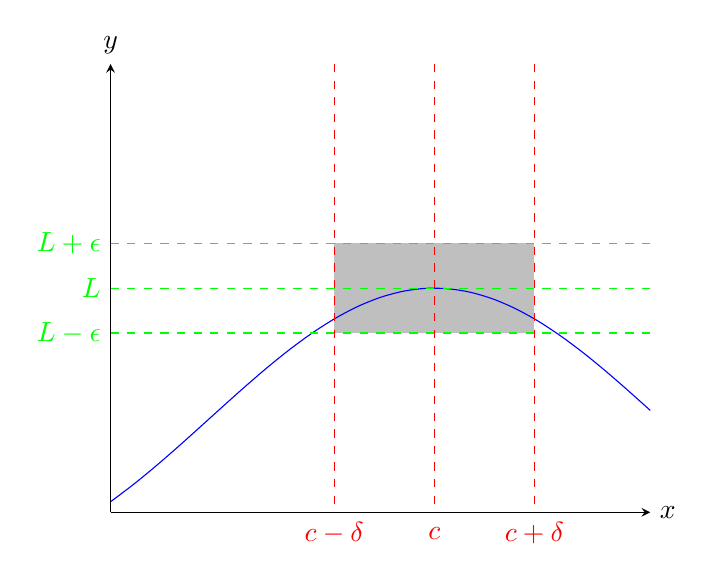
\begin{tikzpicture}
    \begin{axis}[
        axis lines=middle,
        xmin=0,
        xmax=5,
        ymin=0,
        ymax=2,
        ticks=none,
        xlabel={\(x\)},
        ylabel={\(y\)},
        x label style={at={(axis cs:5,0)},anchor=west},
        y label style={at={(axis cs:0,2)},anchor=south},
        clip=false
      ]
      \fill [lightgray] (3-0.9273,0.8) -- (3+0.9273,0.8) -- (3+0.9273,1.2) -- (3-0.9273,1.2) -- cycle;
      \addplot [domain=0:5,blue,smooth] {(sin(deg(x-3)))/(x-3)};
      \draw [dashed,green] (5,1.2) -- (0,1.2) node [left] {\(L+\e\)};
      \draw [dashed,green] (5,1) -- (0,1) node [left] {\(L\)};
      \draw [dashed,green] (5,0.8) -- (0,0.8) node [left] {\(L-\e\)};
      \draw [dashed,red] (3-0.9273,2) -- (3-0.9273,0) node [below] {\(c-\d\)};
      \draw [dashed,red] (3,2) -- (3,0) node [below=0.5ex] {\(c\)};
      \draw [dashed,red] (3.9273,2) -- (3.9273,0) node [below] {\(c+\d\)};
    \end{axis}
  \end{tikzpicture}
\end{center}

Select an \(\e>0\) and then find a \(\d>0\) such that \(f(x)\) is contained in the bounding box.  As \(\e\to0\),
this forces \(\d\to0\) and the bounding box converges to the point \((c,L)\).  This does not imply that \(f(c)=L\).
In fact since \(\abs{x-c}>0\), \(x\ne c\) so we don't care what actually happens at \(x=c\).

\end{document}
